\documentclass[conference]{IEEEtran}
%\IEEEoverridecommandlockouts
% The preceding line is only needed to identify funding in the first footnote. If that is unneeded, please comment it out.
%Template version as of 6/27/2024

\usepackage{cite}
\usepackage{amsmath,amssymb,amsfonts}
\usepackage{algorithmic}
\usepackage{graphicx}
\usepackage{textcomp}
\usepackage{xcolor}
\def\BibTeX{{\rm B\kern-.05em{\sc i\kern-.025em b}\kern-.08em
    T\kern-.1667em\lower.7ex\hbox{E}\kern-.125emX}}
\begin{document}

\title{Automatic Differentiation in Julia: Design and Comparative Performance Evaluation\\
% {\footnotesize \textsuperscript{*}Note: Sub-titles are not captured for https://ieeexplore.ieee.org  and
% should not be used}
% \thanks{Identify applicable funding agency here. If none, delete this.}
}

\author{\IEEEauthorblockN{1\textsuperscript{st} Oliwier Kniażewski}
\IEEEauthorblockA{\textit{Faculty of Electrical Engineering} \\
\textit{Warsaw University of Technology}\\
Warsaw, Poland \\
01169511@pw.edu.pl}
% \and
% \IEEEauthorblockN{2\textsuperscript{nd} Given Name Surname}
% \IEEEauthorblockA{\textit{dept. name of organization (of Aff.)} \\
% \textit{name of organization (of Aff.)}\\
% City, Country \\
% email address or ORCID}
% \and
% \IEEEauthorblockN{3\textsuperscript{rd} Given Name Surname}
% \IEEEauthorblockA{\textit{dept. name of organization (of Aff.)} \\
% \textit{name of organization (of Aff.)}\\
% City, Country \\
% email address or ORCID}
% \and
% \IEEEauthorblockN{4\textsuperscript{th} Given Name Surname}
% \IEEEauthorblockA{\textit{dept. name of organization (of Aff.)} \\
% \textit{name of organization (of Aff.)}\\
% City, Country \\
% email address or ORCID}
% \and
% \IEEEauthorblockN{5\textsuperscript{th} Given Name Surname}
% \IEEEauthorblockA{\textit{dept. name of organization (of Aff.)} \\
% \textit{name of organization (of Aff.)}\\
% City, Country \\
% email address or ORCID}
% \and
% \IEEEauthorblockN{6\textsuperscript{th} Given Name Surname}
% \IEEEauthorblockA{\textit{dept. name of organization (of Aff.)} \\
% \textit{name of organization (of Aff.)}\\
% City, Country \\
% email address or ORCID}
}

\maketitle

\begin{abstract}
Automatic Differentiation (AD) is a critical component in modern machine learning, 
optimization, and scientific computing applications. 
While established frameworks such as TensorFlow, PyTorch, 
and JAX offer robust AD solutions, Julia's emerging ecosystem presents unique opportunities 
for high-performance differentiation leveraging its Just-In-Time (JIT) compilation and 
type system. This work presents the design and implementation of a minimal AD library 
in Julia, focusing on reverse-mode automatic differentiation. 
Optimization strategies, including minimizing memory allocations, 
leveraging multiple dispatch, and explicit variable typing, are employed to 
maximize performance. A comparative evaluation is conducted against popular 
Python-based AD frameworks. The results highlight the potential of Julia for 
delivering efficient, flexible, and scalable AD solutions, contributing to the 
broader adoption of Julia in scientific and machine learning domains.
\end{abstract}

\begin{IEEEkeywords}
automatic differentiation, Julia language, reverse-mode differentiation, machine learning, 
scientific computing, neural networks.
\end{IEEEkeywords}

\section{Introduction}
Julia is a high-level, high-performance programming language designed for numerical 
and scientific computing. Its main advantges include Just-In-Time (JIT) compilation via LLVM, 
which enables executions speeds comparable to C, while maintaining a high-level syntax. 
Automatic Differentiation (AD) is a core computational tool used in optimization, 
machine learning, and scientific simulations. There are two primary modes of AD:

\begin{itemize}
    \item \textbf{Forward Mode}: Computes the derivative of a function as it evaluates the function itself. 
    It is efficient for functions with a small number of inputs and many outputs.
    \item \textbf{Reverse Mode}: Computes the derivative of a function by first evaluating the function and then 
    applying the chain rule in reverse order. It is particularly efficient for functions with many inputs and few outputs, 
    making it ideal for training neural networks.
\end{itemize}

Despite these advantages, effectively leveraging Julia's capabilities for robust 
and performant AD across diverse computational tasks presents unique challenges and 
research opportunities.

\section{Research Context and Importance}

Automatic Differentiation (AD) \cite{b6} is a fundamental technique in machine learning and 
numerical computing. Major frameworks such as TensorFlow \cite{b7}, PyTorch \cite{b3}, 
and JAX integrate efficient AD engines optimized for deep learning tasks. Julia, 
designed for high-performance scientific computing, also offers powerful AD tools 
like ForwardDiff.jl, ReverseDiff.jl, and Zygote.jl. However, 
effectively leveraging Julia's capabilities for robust and performant AD across 
diverse computational tasks presents unique challenges and research opportunities. 
While Julia's AD libraries provide essential functionality, 
they exhibit varying performance and usability challenges that highlight the need for 
further development and evaluation, particularly in comparison to established, 
highly optimized frameworks in other languages.

\section{Summary of Key Studies and Identified Gaps}

\subsection{Literature Review}
This section reviews existing AD tools in Julia, presents relevant performance data, 
and identifies key research gaps.

\subsection{Overwiew of Existing Julia AD Tools}
Julia's high-performance capabilities make it a promising platform for AD. Key libraries 
include \texttt{ForwardDiff.jl} for forward-mode AD, efficient for low-dimensional inputs 
but less scalable for high-dimensional problems. \texttt{ReverseDiff.jl} \cite{b8} 
employs a tape-based reverse-mode AD, suitable for many inputs and few outputs, 
but can incur overheads due to graph recording. \texttt{Zygote.jl} \cite{b9} uses source-to-source 
transformation for flexible reverse-mode AD, capable of handling complex Julia features, 
but faces performance challenges with dynamic graph transformation and array mutations.

\subsection{Performance Benchamrks}
Empirical performance evaluation is essential for understanding the practical 
capabilities of AD tools and identifying ares for improvement. While comprehesive, 
standardized benchmarks are limited, existing studies provide valuable insights. For 
instance, benchmarks comparing Julia-based AD libraries against established Python 
frameworks like PyTorch on specific tasks have shown that Julia's tools can offer 
significant performance advantages, as illustratesd in Table \ref{tab:benchmark}:

\begin{table}[ht]
    \caption{Benchmark Results \cite{b1}}
    \centering
    \scriptsize
    \begin{tabular}{lcccc}
    \hline
    \textbf{Benchmark} & \textbf{Forward} & \textbf{Zygote} & \textbf{PyTorch} & \textbf{ReverseDiff} \\
    \hline
    SINCOS & 15.9 ns & 20.7 ns & 69,900 ns & 670 ns \\
    LOOP & 4.17 $\mu$s & 29.5 $\mu$s & 17,500 $\mu$s & 171 $\mu$s \\
    LOGSUMEXP & 0.96 $\mu$s & 1.26 $\mu$s & 219 $\mu$s & 15.9 $\mu$s \\
    LOGISTIC REGRESSION & 4.67 $\mu$s & 17.6 $\mu$s & 142 $\mu$s & 89.9 $\mu$s \\
    2-LAYER MNIST MLP & 27.7 $\mu$s & 207 $\mu$s & 369 $\mu$s & N/A \\
    \hline
    \end{tabular}
    \label{tab:benchmark}
\end{table}

These results indicate that Julia AD libraries generally outperform PyTorch on these 
specific tasks, demonstrating Julia's potential. However, they also show varying performance 
characteristics among Julia libraries and highlight areas where overhead is significant 
compared to a manual forward pass.

Furthermore, performance comparisons are not limited to high-level frameworks. Studies 
evaluating Julia's AD tools against traditional compiled languages like C++ in specific 
scenarios reveal compelling performance characteristics. This suggests that for certain 
computational patterns, leveraging Julia's AD capabilities can yield performance 
superior even to straightforward manual implementations in C++, highlighting the 
effectiveness of Julia's JIT compilation and AD infrastructure. 
This underscores the need for further comprehensive performance analysis and optimization.

\begin{table}[ht]
    \caption{Rosenbrock and Ackley gradient evalutation times (input size 12000) \cite{b1}}
    \centering
    \scriptsize
    \begin{tabular}{lcc}
    \hline
    \textbf{chunk size N} & \textbf{C++ Time} & \textbf{ForwardDiff Time} \\
    \hline
    1 & 2.66744 s & 0.62760 s \\
    2 & 2.71184 s & 0.45541 s \\
    3 & 1.92713 s & 0.44469 s \\
    4 & 1.45306 s & 0.42354 s \\
    5 & 1.24949 s & 0.44045 s \\
    \hline
    \end{tabular}
    \label{tab:comparison}
\end{table}

\section{Justification for the Proposed Research}
Despite active development, Julia's AD solutions lack comprehensive performance
evaluations across a wide range of tasks relative to established Python frameworks.
This research aims to address this gap by:
\begin{itemize}
    \item Implementing a minimal AD library in Julia, focusing on reverse-mode differentiation,
    \item applying Julia-specific optimization strategies, including:
    \begin{itemize}
        \item Minimizing memory allocations,
        \item leveraging multiple dispatch,
        \item explicit variable typing.
    \end{itemize}
    \item Conducting a comparative evaluation against popular Python-based AD framework.
\end{itemize}
The goal is to highlight the potential of Julia for delivering efficient, flexible,
and scalable AD solutions, contributing to the broader adoption of Julia in scientific
and machine learning domains.

\section{Conclusions from Literature Analysis and Research Implications}
The current literature reveals Julia's potential for high-performance AD but 
also identifies critical bottlenecks, including type instability, memory overhead, 
and lack of standardized benchmarking.

This study aims to deliver both practical insights and empirical data for advancing 
Julia's competitiveness in the automatic differentiation ecosystem, 
with direct implications for machine learning, optimization, 
and scientific computing applications.

\section{Implementation idea}
To implement the project, a backpropagation approach based on a computational graph was chosen. The layers consist of one or more nodes, which serve as components of the computation (Variables and Constants) or represent operations (Operators). Each operator has a forward function (to compute the result) and a backward function (to compute the gradient). Once the graph is created, it undergoes topological sorting, which facilitates both forward and backward passes.

In order to enable comparison with existing machine learning libraries, a custom module was developed. 

The project consists of three modules:

\begin{itemize}
    \item \textbf{MyReverseDiff} – Defines the structure of the graph, node types, and the forward and backward pass operations.
    \item \textbf{MyMLP} – Defines the layers, the structure of the neural network, and optimizers (e.g., ADAM).
    \item \textbf{MyEmbedding} – Describes embedding operations.
\end{itemize}

\section{Difficulties during project}
???

\section{Implemented optimization}
???

\section{Tests}
Technologies used for comparison are PyTorch (Python) and Flux (Julia).

\subsection{Used network architecture}

For comparison purposes, a Convolutional Neural Network (CNN) was chosen. Its task is to classify reviews as positive or negative based on their text. The reviews are sourced from the IMDB website.

The network is built using six layers. The first is a preprocessed embedding layer based on GloVe. The second layer swaps the first and second dimensions of the input tensor. The third layer is a convolutional layer that processes the input using 8 filters of size 3×50, followed by a ReLU activation function. The next layer is a max pooling layer that reduces the first dimension by a factor of eight. The fifth layer is a flattening layer. The final layer is a dense layer that reduces the vector to a scalar and passes it through a sigmoid function.

The network input consists of 64 reviews. Each review is a vector of 130 words, represented as indices in the embedding dictionary. The output is 64 values in the range [0, 1], representing whether the reviews are classified as positive or negative. \ref{fig:Network_architecture}

\begin{figure}
    \centering
    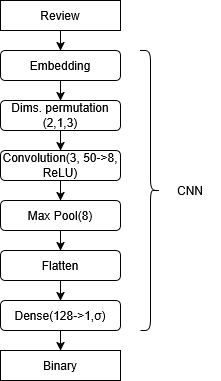
\includegraphics[height=0.9\linewidth]{Network.png}
    \caption{Network architecture}
    \label{fig:Network_architecture}
\end{figure}

\subsection{Correctness tests}
???

\subsection{Efficienty tests}
???

\section{Results}
??? Tests results

\subsection{Limitations}

In its current state, the project allows for the creation of CNN and MLP networks, but with a very limited selection of activation functions. Creating other types of networks would require users to manually implement the layers as well as the forward and backward operations. Optimizers also pose a limitation, as the only available options are Gradient Descent and ADAM.

\subsection{Possible development directions}
There are two possible directions for the further development of the project. The first is to improve performance by reducing memory allocation and decreasing training time. This would require continued work on code optimization.
Another development path is to expand the functions and operators supported by the AD (Automatic Differentiation) library. Increasing the number of activation functions and adding operations essential for other neural network architectures (e.g., RBF, RNN, etc.) would significantly broaden the library's applicability and make it suitable for use in other projects.

\begin{thebibliography}{00}
\bibitem{b1} M. J. Innes, ``DON'T UNROLL ADJOINT: DIFFERENTIATING SSA-FORM PROGRAMS,'' 2019, arXiv:1810.07951. [Online]. Available: https://arxiv.org/abs/1810.07951
\bibitem{b2} L. Hascoët, U. Naumann, and V. Pascual, ``"To be recorded" analysis in reverse-mode automatic differentiation,'' Future Generation Computer Systems, vol. 21, pp. 1401--1417, 2005. doi: 10.1016/j.future.2004.11.009.
\bibitem{b3} A. Paszke, G. Chanan, Z. Lin, S. Gross, S. Chintala, E. Yang, L. Antiga, Z. DeVito, A. Lerer, and A. Desmaison, ``Automatic differentiation in PyTorch,'' in 31st Conference on Neural Information Processing Systems (NIPS 2017), Long Beach, CA, USA, 2017.
\bibitem{b4} J. Revels, M. Lubin, and T. Papamarkou, ``Forward-Mode Automatic Differentiation in Julia,'' 2016, arXiv:1607.07892. [Online]. Available: https://arxiv.org/abs/1607.07892
\bibitem{b5} C. C. Margossian, ``A Review of Automatic Differentiation and its Efficient Implementation,'' 2019, arXiv:1811.05031. [Online]. Available: https://arxiv.org/abs/1811.05031
\bibitem{b6} Y.-H. Fang, H.-Z. Lin, J.-J. Liu, and C.-J. Lin, ``A Step-by-step Introduction to the Implementation of Automatic Differentiation,'' 2024, arXiv:2402.16020. [Online]. Available: https://arxiv.org/abs/2402.16020
\bibitem{b7} M. Abadi et al., ``TensorFlow: Large-Scale Machine Learning on Heterogeneous Distributed Systems,'' 2016, arXiv:1603.04467. [Online]. Available: https://arxiv.org/abs/1603.04467
\bibitem{b8} M. Innes, ``ReverseDiff.jl,'' 2018. [Online]. Available: https://github.com/JuliaDiff/ReverseDiff.jl
\bibitem{b9} M. Innes et al., ``Zygote.jl,'' 2018. [Online]. Available: https://fluxml.ai/Zygote.jl/latest/
\bibitem{b10} M. Innes et al., ``Flux: Elegant Machine Learning with Julia,'' Journal of Open Source Software, vol. 3, no. 25, p. 602, 2018, doi: 10.21105/joss.00602.
\end{thebibliography}

\end{document}
